\section{Architettura del prodotto}
Dopo un approfondito studio il team ha optato per l'utilizzo del design pattern \textbf{Model View View-Model}, che prevede tre macrosezioni:
	\begin{itemize}
		\item \textbf{Model}: rappresenta i dati contenuti nel sito, ma non i comportamenti o i servizi che manipolano l'informazione. Non è responsabile della renderizzazione;
		\item \textbf{View}: si occupa di rappresentare le informazioni contenute nel sito ed è quello con cui l'utente interagisce; la view in questo design pattern è attiva, al contrario di quello che succede nell'MVC, questo perché contiene comportamenti, eventi e riferimenti a stati del sito, che quindi presuppongo una conoscenza della logica che sta dietro ai dati;
		\item \textbf{Viewmodel}: fornisce i dati dal Model in una forma in cui la View può usufruirne. Si occupa inoltre della logica della vista e di mantenersi costantemente sincronizzato con la View.
	\end{itemize}
Per poter apprezzare questa suddivisione nel pacchetto del team viene riportato qui di seguito il diagramma generale dei package. Si proseguirà successivamente alla descrizione delle implementazioni di ogni sezione in relazione all'architettura della Product Baseline, illustrandone i rispettivi design pattern utilizzati.
\\Per facilitare la comprensione della struttura dei diagrammi delle classi, il team ha deciso di raggruppare tutti i \emph{Containers}, i \emph{Components} e le \emph{actions} nei loro rispettivi packages. Infatti il comportamento di ogni classe di ogni package è modulare:
	\begin{itemize}
		\item Tutti i \emph{Components} importano la classe \emph{React.Component}
		\item Tutti i \emph{Containers} importano il rispettivo \emph{Component}, la rispettiva \emph{Action} e il pacchetto \emph{react-redux}.
		\item Tutte le \emph{actions} importano le \emph{costants} che azionano il \emph{reducer}, il pacchetto \emph{react-router}, lo \emph{store}, il pacchetto \emph{truffle-contract} e la classe \emph{IpfsUtils}
	\end{itemize}
I diagrammi presentati in questo documento illustrano la struttura sinteticamente; la loro versione integrale si può trovare nella cartella {\textcolor{red}{INSERIRE LA CARTELLA}}.

{\textcolor{red}{INSERIRE DIAGRAMMA DEI PACKAGE IN GENERALE}}
\begin{figure}[h]
	\centering
%	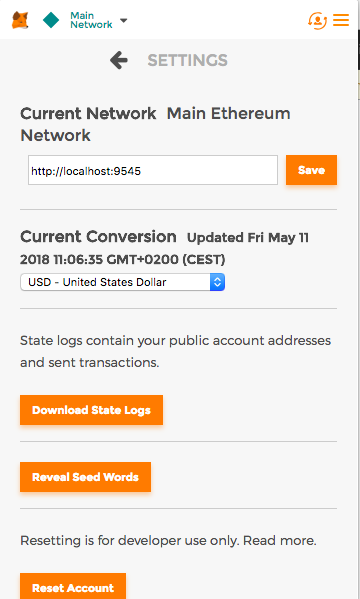
\includegraphics[height=3in]{./img/settings.png}
	\caption{Diagramma generale dei package}
	\label{}
\end{figure}

	\subsection{Model}
		\subsubsection{Design patterns}
		Per quanto riguarda la macrosezione relativa alla componente Model, si sono utilizzati i seguenti design pattern: {\textcolor{red}{INSERIRE I PATTERN}}
			\begin{itemize}
				\item \textbf{}: ;
				\item \textbf{}: .
				\item \textbf{}: .
			\end{itemize}
		
		\subsubsection{Diagramma delle classi}
		In seguito è riportato il diagramma delle classi relativo a questa sezione con evidenziato la posizione del design pattern utilizzato.
	
	{\textcolor{red}{INSERIRE DIAGRAMMA CON VISTA SU MODEL}}
	\begin{figure}[h]
		\centering
		%	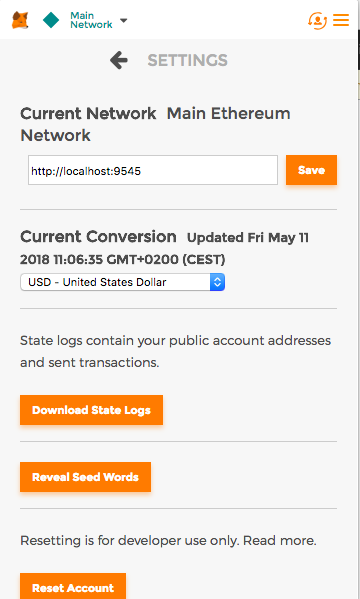
\includegraphics[height=3in]{./img/settings.png}
		\caption{Diagramma delle classi del componente Model}
		\label{}
	\end{figure}
	
	\subsection{View}
		\subsubsection{Design patterns}
		Progettando questa sezione ci si è resi conto che si sarebbero potute generare delle classi \emph{dumb}, ovvero slegate dalla logica del sistema e che si sarebbero dovute occupare solamente della rappresentazione delle informazioni. Per ottenere questo si è ricorso all'utilizzo del seguente design pattern:
			\begin{itemize}
				\item \textbf{Decorator}: sfruttando il macro-package \emph{Container}, che poi si occupa di collegare il componente allo stato di \emph{redux}, si possono decorare tutte le componenti ivi presenti con dei componenti react puri, ai quali vengono passate eventualmente le informazioni e le funzioni a disposizione attraverso un accesso al \emph{this.props}. In questa maniera si ha la completa separazione tra rappresentazione e dati - cosa auspicata dal framework MVVM - e si facilitano modifiche future.
			\end{itemize}
		
		\subsubsection{Diagramma delle classi}
		In seguito è riportato il diagramma delle classi relativo a questa sezione con evidenziato la posizione del design pattern utilizzato.
	
	{\textcolor{red}{INSERIRE DIAGRAMMA CON VISTA SU VIEW}}
	\begin{figure}[h]
		\centering
		%	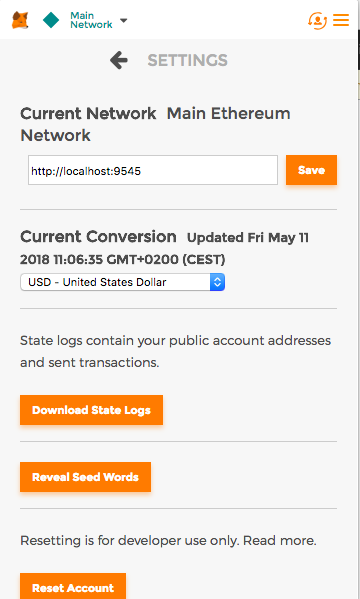
\includegraphics[height=3in]{./img/settings.png}
		\caption{Diagramma delle classi del componente View}
		\label{}
	\end{figure}
	
	\subsection{ViewModel}
		\subsubsection{Design patterns}
		Per la sezione riguardante il ViewModel, si è ricorso all'utilizzo dei seguenti design pattern:
			\begin{itemize}
				\item \textbf{Observer}: descrizione per quanto riguarda il comportamento di trigger-client che opera Redux sullo stato di React;
				\item \textbf{Façade}: per generare un'interfaccia astratta dalle implementazioni delle classi che poi si vanno ad utilizzare;
				\item \textbf{Adapter}: per interagire col model si usa un adaptator offerto dal framework truffle che si occupa di {\textcolor{red}{fare-un-sacco-di-cose-belle-da-chiedere-a-Stefano}};
				\item \textbf{Command}: come redux ordina a react di re-renderizzare le pagine al cambiamento dello state dovuto ad un dispatch di un'azione.
			\end{itemize}
	
		\subsubsection{Diagramma delle classi}
		In seguito è riportato il diagramma delle classi relativo a questa sezione con evidenziato la posizione del design pattern utilizzato.
	
	{\textcolor{red}{INSERIRE DIAGRAMMA CON VISTA SU VIEWMODEL}}
	\begin{figure}[h]
		\centering
		%	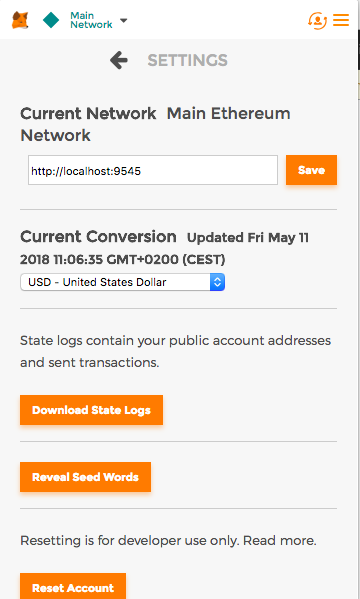
\includegraphics[height=3in]{./img/settings.png}
		\caption{Diagramma delle classi del componente ViewModel}
		\label{}
	\end{figure}
	
	\subsection{Diagrammi di sequenza}
	Come per i diagrammi delle classi, sono stati redatti i seguenti diagrammi di sequenza, disponibili e meglio visualizzabili nella cartella {\textcolor{red}{INSERIRE LA CARTELLA}};
	
		\subsubsection{Login}
		Il diagramma di sequenza riportato qui di seguito raffigura il processo di login, durante il quale l'utente che vuole accedere può essere autenticato dal sistema.
		{\textcolor{red}{INSERIRE DIAGRAMMA DI LOGIN}}
		\begin{figure}[h]
			\centering
			%	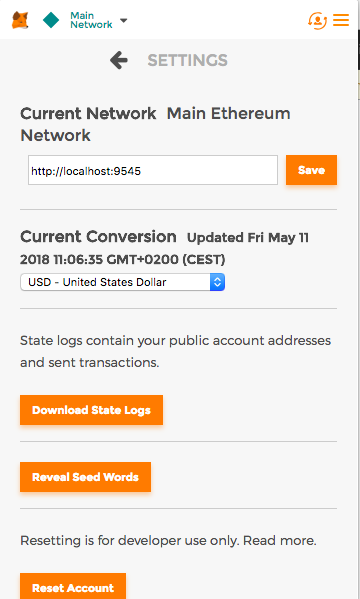
\includegraphics[height=3in]{./img/settings.png}
			\caption{Diagramma di sequenza del processo di login}
			\label{}
		\end{figure}
		
		\subsubsection{Inserimento di un utente}
		Il seguente diagramma di sequenza rappresenta l'azione di inserimento di un utente nel sistema.
		{\textcolor{red}{INSERIRE DIAGRAMMA DI INSERIMENTO UTENTE}}
		\begin{figure}[h]
			\centering
			%	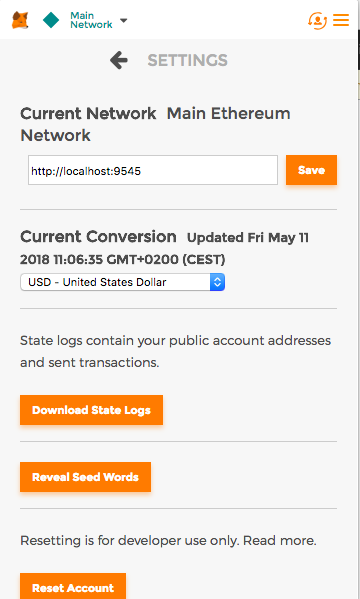
\includegraphics[height=3in]{./img/settings.png}
			\caption{Diagramma di sequenza del processo di inserimento di un utente}
			\label{}
		\end{figure}
		
		\subsubsection{Inserimento di un anno accademico}
		Il diagramma di sequenza riportato qui di seguito raffigura il processo di inserimento di un nuovo anno accademico nel sistema.
		{\textcolor{red}{INSERIRE DIAGRAMMA DI INSERIMENTO ANNO ACCADEMICO}}
		\begin{figure}[h]
			\centering
			%	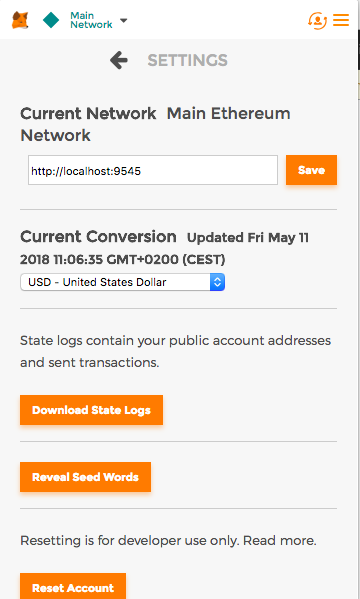
\includegraphics[height=3in]{./img/settings.png}
			\caption{Diagramma di sequenza del processo di inserimento di un anno accademico}
			\label{}
		\end{figure}
		
		\subsubsection{Visualizzazione di un anno accademico}
		Il seguente diagramma di sequenza rappresenta l'azione di visualizzazione di un anno accademico.
		{\textcolor{red}{INSERIRE DIAGRAMMA DI VISUALIZZAZIONE ANNO ACCADEMICO}}
		\begin{figure}[h]
			\centering
			%	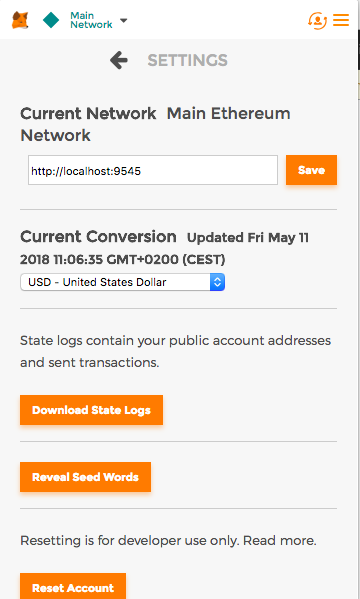
\includegraphics[height=3in]{./img/settings.png}
			\caption{Diagramma di sequenza del processo di visualizzazione di un anno accademico}
			\label{}
		\end{figure}
	
	
	
	
	